% !TeX root = ../bbchallenge-paper.tex

\newpage
\subsection{Weighted FAR (WFAR)}\label{sec:WFAR}

% 1RB---_0RC1LC_1RD1RC_1LE1LD_0RA0LE
% 1RB---_0RC1LB_1RD1RC_1LE1LD_0RA0LE
% 1RB---_0RC1RC_1RD1RC_1LE1LD_0RA0LE
% 1RB---_0RC1RC_1RD1RB_1LE1LD_0RA0LE *
% 1RB1RA_1LC1LB_0RD0LC_1RE---_0RA1RA
% 1RB1RA_1LC1LB_0RD0LC_1RE---_0RA1LA
% 1RB1RA_1LC1LB_0RD0LC_1RE---_0RA1LE
% 1RB1RE_1LC1LB_0RD0LC_1RE---_0RA1RA
% 1RB1RA_1LC1LE_0RD0LC_1RE---_0RA1LB
% 1RB---_0RC1LD_1RD1RC_1LE1LB_0RA0LE
% 1RB1RE_1LC1LB_0RD0LC_1LE---_0RA1RA
% 1RB---_0LC1LC_1LD1LB_1RE1RD_0LA0RE
% 1RB1LC_1LC1RA_0LE0LD_0RA1RD_---0LC *
% 1RB1LC_1LB1RA_0LE0LD_0RA1RD_---0LC
% 1RB0RC_1LC0LE_0LD0LB_1RA---_1LB0RD
% 1RB0RE_0RC0RA_1LD---_1LA0LB_1RA0LC
% 1RB0LD_1RC0RA_0RD0RB_1LE---_1LB0LC *
\usetikzlibrary{automata, positioning, arrows.meta}
\begin{figure}[h!]
    \centering
    \begin{minipage}[t]{0.23\textwidth}
        \raggedright
        (a) Turing machine \\
        \centering
        \vspace{0.6em}
        \begin{tabular}{ccc}
            \toprule
                    & \textbf{0} & \textbf{1} \\
            \midrule
            \stateA & 1R\stateB  & ---        \\
            \stateB & 0R\stateC  & 1L\stateC  \\
            \stateC & 1R\stateD  & 1R\stateC  \\
            \stateD & 1L\stateE  & 1L\stateD  \\
            \stateE & 0R\stateA  & 0L\stateE  \\
            \bottomrule
        \end{tabular}

        \vspace{0.8em}
        \raggedright
        (a') Space-time diagram \\
        \vspace{0.3em}
        \centering
        \includegraphics[width=1.1\linewidth]{figures/space-time-diagrams/counter_wfar.png}

        % \vspace{0.8em}
        % \raggedright
        % (a') Space-time diagram \\
        % \vspace{0.3em}
        % \centering
        % \includegraphics[width=1.1\linewidth]{figures/wfar/wfar_example.pdf}
    \end{minipage}
    \hfill
    \vrule
    \hfill
    \begin{minipage}[t]{0.71\textwidth}

        \begin{minipage}[t]{1\linewidth}

            \begin{minipage}[t]{0.49\textwidth}
                \raggedright
                (b) Left Weighted Automaton \\
                \vspace{0.5em}
                \centering
                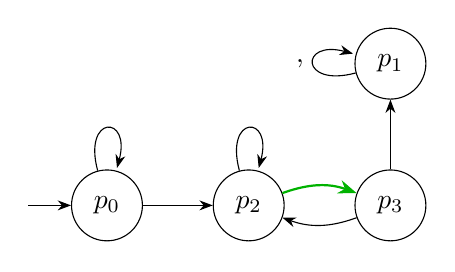
\begin{tikzpicture}[->, >=Stealth, auto, node distance=1.8cm, every node/.style={scale=1}]
                    \tikzset{
                        state/.style={
                                circle, draw, minimum size=0.9cm, inner sep=1pt
                            }
                    }

                    % States
                    \node[state] (0) {$p_0$};
                    \node[state] (2) [right of=0] {$p_2$};
                    \node[state] (3) [right of=2] {$p_3$};
                    \node[state] (1) [above of=3] {$p_1$};

                    % Initial arrow
                    \draw[->] (-1,0) -- (0);

                    % Transitions
                    \draw[->, black] (0) edge[loop above] node{\szero} (0);
                    \draw[->, black] (0) edge node{\sone} (2);

                    \draw[->, black] (2) edge[loop above] node{\sone} (2);
                    \draw[->, black, bend left=20] (3) to node{\sone} (2);
                    \draw[->, green!70!black, thick, bend left=20] (2) to node{\szero} (3);

                    \draw[->, black] (3) edge node{\szero} (1);
                    \draw[->, black] (1) edge[loop left] node{\szero, \sone} (1);


                \end{tikzpicture}
            \end{minipage}
            \hfill
            \begin{minipage}[t]{0.49\textwidth}
                \raggedright
                (c) Right Weighted Automaton \\
                \vspace{0.3em}
                \centering
                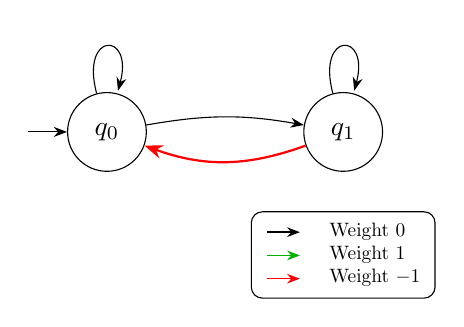
\begin{tikzpicture}[->, >=Stealth, auto, node distance=2cm, every node/.style={scale=1}]
                    \tikzset{
                        state/.style={
                                circle, draw, minimum size=1cm, inner sep=1pt
                            }
                    }

                    % % Upper isolated state
                    % \node[state] (1top) at (0,2.5) {1};
                    % \draw[->] (1top) edge[loop above] node{1} (1top);
                    % \draw[->] (1top) edge[loop left] node{0} (1top);

                    % Lower automaton
                    \node[state] (0) at (0,0) {$q_0$};
                    \node[state] (2) at (3,0) {
                        $q_1$};

                    \draw[->] (0) edge[loop above] node{\szero} (0);
                    \draw[->] (2) edge[loop above] node{\sone} (2);

                    \draw[->] (0) edge[bend left=10] node{\sone} (2);
                    \draw[->, red, bend left=20, thick] (2) to node[below]{\szero} (0);

                    % Initial state arrow
                    \draw[->] (-1,0) -- (0);

                    % Compact and aligned legend
                    \node[draw, below=0.5cm of 2, inner sep=3pt, rounded corners] (legend) {
                        \scalebox{0.7}{
                            \begin{tabular}{@{}rl@{}}
                                \tikz[baseline=-0.5ex]\draw[->, black, thick] (0,0) -- +(0.6,0);          & \;Weight 0    \\
                                \tikz[baseline=-0.5ex]\draw[->, green!70!black, thick] (0,0) -- +(0.6,0); & \;Weight 1    \\
                                \tikz[baseline=-0.5ex]\draw[->, red, thick] (0,0) -- +(0.6,0);            & \;Weight $-1$
                            \end{tabular}
                        }
                    };
                \end{tikzpicture}
            \end{minipage}

            % \vspace{1em}
            % $\rightarrow$ \quad 1\,0\,|\,0\,|\,0\,1 \\
            % \vspace{0.5em}
            % $+\;4$

        \end{minipage}

        \vspace{1em}

        \raggedright
        (d) Example: configuration is accepted, hence nonhalting \\
        \vspace{0.3em}
        \centering

        \newcommand{\underarrowleft}[1]{%
            \tikz[baseline=(X.base)]{
                \node (X) {$#1$};
                \draw[->, thick] ([yshift=-1.3ex]X.east) -- ([yshift=-1.3ex]X.west);
            }
        }

        \newcommand{\underarrowright}[1]{%
            \tikz[baseline=(X.base)]{
                \node (X) {$#1$};
                \draw[->, thick] ([yshift=-1.3ex]X.west) -- ([yshift=-1.3ex]X.east);
            }
        }

        \scalebox{0.8}{

            \begin{minipage}{\textwidth}
                \centering
                {\LARGE
                $\underarrowright{\texttt{10101}}\; \texttt{\stateC}\sone\; \underarrowleft{\texttt{01}}$ \\
                \vspace{-0.3em}
                {\small $\quad\quad$Left WA reads$\quad\quad\quad\quad\quad\quad\quad\quad$Right WA reads} \\
                %\vspace{0.1em}
                $\quad  \; \;$\fcolorbox{red}{yellow!30}{$[p_2] \; \texttt{\stateC}\sone\; [q_0]$} \\
                \vspace{-2em}
                \[
                    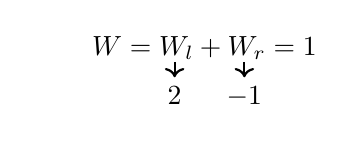
\begin{tikzpicture}[baseline=(base)]
                        \node (base) {$\quad \quad W = W_l + W_r = 1$};

                        \coordinate (Wl) at ([xshift=5.33em]base.base west);
                        \coordinate (Wr) at ([xshift=7.85em]base.base west);

                        % Labels
                        \node[below=1.8ex of Wl] (lval) {\normalsize 2};
                        \node[below=1.8ex of Wr] (rval) {\normalsize $-1$};

                        % Arrows pointing down from W_l and W_r
                        \draw[->, thick] ([yshift=-0.5ex]Wl) -- (lval.north);
                        \draw[->, thick] ([yshift=-0.5ex]Wr) -- (rval.north);
                    \end{tikzpicture}
                \] \\
                \vspace{-0.5em}
                {\large Configuration accepted, see (e), hence machine does not halt starting from $\texttt{10101}\; \texttt{\stateC}\sone\; \texttt{01}$, see Theorem~\ref{th:WFAR}. }
                }
                % \begin{tikzpicture}[->, >=Stealth, auto, node distance=2cm, every node/.style={scale=1}]
                %     \tikzset{
                %         state/.style={
                %                 circle, draw, minimum size=1cm, inner sep=1pt
                %             }
                %     }

                %     % % Upper isolated state
                %     % \node[state] (1top) at (0,2.5) {1};
                %     % \draw[->] (1top) edge[loop above] node{1} (1top);
                %     % \draw[->] (1top) edge[loop left] node{0} (1top);

                %     % Lower automaton
                %     \node[state] (0) at (0,0) {0};
                %     \node[state] (2) at (3,0) {1};

                %     \draw[->] (0) edge[loop above] node{0} (0);
                %     \draw[->] (2) edge[loop above] node{1} (2);

                %     \draw[->] (0) edge[bend left=10] node{1} (2);
                %     \draw[->, red, bend left=20, thick] (2) to node[below]{0} (0);

                %     % Initial state arrow
                %     \draw[->] (-1,0) -- (0);
                % \end{tikzpicture}
            \end{minipage}
        }

        \vspace{0.5em}
        \raggedright
        (e) Accepted weighted configurations \\
        \centering

        \usetikzlibrary{positioning, shapes.multipart, fit}
        \scalebox{0.8}{
            \begin{tikzpicture}[node distance=0.2cm and 0.3cm, every node/.style={font=\normalsize}, anchor=north]

                % Reference coordinate for top alignment
                \coordinate (topref) at (0,0);

                % W >= -1 group
                \node[draw, rectangle, rounded corners, inner sep=3pt] (wmin1box)
                {\begin{tabular}{l}
                        $[p_2]\; \texttt{\stateE}\szero\; [q_0]$
                    \end{tabular}};
                \node[above=0cm of wmin1box] {$W \geq$ -1};

                % W = 0 group
                \node[draw, rectangle, rounded corners, inner sep=3pt, right=of wmin1box] (w0box)
                {\begin{tabular}{l}
                        $[p_0]\; \texttt{\stateA}\szero\; [q_0]$ \\
                        $[p_0]\; \texttt{\stateE}\szero\; [q_0]$ \\
                        $[p_0]\; \texttt{\stateE}\sone\; [q_0]$
                    \end{tabular}};
                \node[above=0cm of w0box] {$W = 0$};

                % W >= 0 group
                \node[draw, rectangle, rounded corners, inner sep=3pt, right=of w0box] (w0plusbox)
                {\begin{tabular}{l}
                        $[p_2]\; \texttt{\stateB}\szero\; [q_0]$ \\
                        $[p_2]\; \texttt{\stateE}\sone\; [q_0]$  \\
                        $[p_3]\; \texttt{\stateE}\sone\; [q_0]$
                    \end{tabular}};
                \node[above=0cm of w0plusbox] {$W\geq0$};
                % W >= 1 group
                \node[draw, rectangle, rounded corners, inner sep=3pt, below=0.6cm of w0box, xshift=1.4cm] (w1box)
                {\begin{tabular}{ll}
                        $[p_3]\; \texttt{\stateA}\szero\; [q_1]$                                             & $[p_2]\; \texttt{\stateC}\sone\; [q_1]$  \\
                        $[p_2]\; \texttt{\stateB}\szero\; [q_1]$                                             & $[p_3]\; \texttt{\stateC}\sone\; [q_1]$  \\
                        $[p_2]\; \texttt{\stateB}\sone\; [q_0]$                                              & $[p_2]\; \texttt{\stateD}\szero\; [q_0]$ \\
                        $[p_2]\; \texttt{\stateB}\sone\; [q_1]$                                              & $[p_2]\; \texttt{\stateD}\szero\; [q_1]$ \\
                        $[p_2]\; \texttt{\stateC}\szero\; [q_0]$                                             & $[p_2]\; \texttt{\stateE}\sone\; [q_1]$  \\
                        $[p_3]\; \texttt{\stateC}\szero\; [q_0]$                                             & $[p_3]\; \texttt{\stateE}\sone\; [q_1]$  \\
                        \rule{0pt}{3.3ex}\fcolorbox{red}{yellow!30}{$[p_2]\; \texttt{\stateC}\sone\; [q_0]$} &                                          \\
                    \end{tabular}};
                \node[above=0cm of w1box] {$W \geq 1$};

                % W >= 2 group
                \node[draw, rectangle, rounded corners, inner sep=6pt, below=0.7cm of wmin1box] (w2box)
                {\begin{tabular}{l}
                        $[p_3]\; \texttt{\stateA}\szero\; [q_0]$ \\
                        $[p_2]\; \texttt{\stateC}\szero\; [q_1]$ \\
                        $[p_3]\; \texttt{\stateC}\szero\; [q_1]$ \\
                        $[p_3]\; \texttt{\stateC}\sone\; [q_0]$  \\
                        $[p_2]\; \texttt{\stateD}\sone\; [q_0]$  \\
                        $[p_2]\; \texttt{\stateD}\sone\; [q_1]$  \\
                        $[p_3]\; \texttt{\stateD}\sone\; [q_1]$  \\
                    \end{tabular}};
                \node[above=0cm of w2box] {$W \geq 2$};

            \end{tikzpicture}
        }
    \end{minipage}

    \caption{{\small WFAR certificate of nonhalting for machine \tm{1RB---_0RC1LC_1RD1RC_1LE1LD_0RA0LE}: (a) transition table and 20,000-step space-time diagram, (b) left weighted automaton: processes symbols to the left of the head in the left-to-right direction, which results in a left end-state -- \eg state $p_2$ when processing \texttt{10101} -- and a left weight obtained by summing the weights of each transition -- \eg $W_l = 2$ when processing \texttt{10101} (c) right weighted automaton: processes symbols to the right of the head (excluding the symbol read by the head) in the right-to-left direction -- indicated with arrow --, which results in a right end-state -- \eg state $q_0$ when processing \texttt{01} right-to-left -- and a right weight -- \eg $W_r = -1$ when processing \texttt{01} right-to-left (d) example, the total weight of configuration $\texttt{10101}\; \texttt{\stateC}\sone\; \texttt{01}$ is $W=W_l+W_r = 1$, using same word-encoding of configurations as in Section~\ref{sec:FAR}, and the right and left end-states are $p_2$ and $q_0$. Weighted automaton configuration $[p_2]\; \texttt{\stateC}\texttt{1}\; [q_0]$ with $W = 1$ is in the set of accepted weighted configurations (under more general $W \geq 1$), see (e). Therefore we know that the machine does not halt from configuration $\texttt{10101}\; \texttt{\stateC}\sone\; \texttt{01}$, Theorem~\ref{th:WFAR}. Similarly, Turing machine configuration $\texttt{\stateA}\texttt{0}$, which results in weighted configuration $[p_0]\;\texttt{\stateA}\texttt{0}\; [q_0]$ with $W=0$ is accepted, ensuring that the machine does not halt from the all-0 initial tape, Theorem~\ref{th:WFAR}.}}\label{fig:WFAR}
\end{figure}

\subsubsection{Overview}\label{sec:WFAR:overview}



\begin{figure}
    \centering
    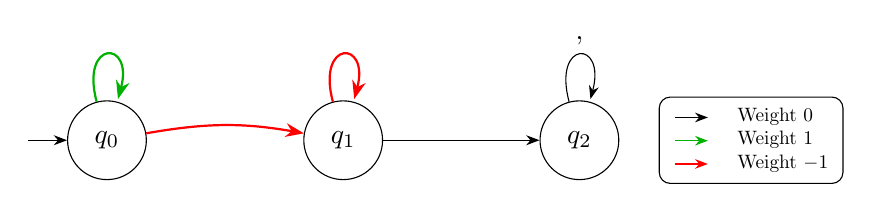
\begin{tikzpicture}[->, >=Stealth, auto, node distance=2cm, every node/.style={scale=1}]
        \tikzset{
            state/.style={
                    circle, draw, minimum size=1cm, inner sep=1pt
                }
        }

        % % Upper isolated state
        % \node[state] (1top) at (0,2.5) {1};
        % \draw[->] (1top) edge[loop above] node{1} (1top);
        % \draw[->] (1top) edge[loop left] node{0} (1top);

        % Lower automaton
        \node[state] (0) at (0,0) {$q_0$};
        \node[state] (2) at (3,0) {$q_1$};
        \node[state] (3) at (6,0) {$q_2$};

        \draw[->, green!70!black, thick] (0) edge[loop above] node{\szero} (0);
        \draw[->, red, thick] (2) edge[loop above] node{\sone} (2);
        \draw[->] (3) edge[loop above] node{\szero,\sone} (3);

        \draw[->, red, thick] (0) edge[bend left=10] node{\sone} (2);
        \draw[->] (2) to node[below]{\szero} (3);

        % Initial state arrow
        \draw[->] (-1,0) -- (0);

        % Compact and aligned legend
        \node[draw, right=0.5cm of 3, inner sep=3pt, rounded corners] (legend) {
            \scalebox{0.7}{
                \begin{tabular}{@{}rl@{}}
                    \tikz[baseline=-0.5ex]\draw[->, black, thick] (0,0) -- +(0.6,0);          & \;Weight 0    \\
                    \tikz[baseline=-0.5ex]\draw[->, green!70!black, thick] (0,0) -- +(0.6,0); & \;Weight 1    \\
                    \tikz[baseline=-0.5ex]\draw[->, red, thick] (0,0) -- +(0.6,0);            & \;Weight $-1$
                \end{tabular}
            }
        };
    \end{tikzpicture}
    \caption{Weighted automaton recognising nonregular language $\texttt{0}^n \texttt{1}^n$, using accept set $\{(q_1,W=0)\}$ or $\{(q_1,W=0), (q_0,W=0)\}$ if we include the empty word.}\label{fig:ex_wa}
\end{figure}

Weighted automata are an extension of usual finite state automata where each transition is given a weight in $\Z$: when a word is processed, total weight $W \in \Z$ is computed by summing the weights of all the encountered transitions. Accepted words are described by a set of pairs of final-state and weigth lower and upper bounds (potentially infinite) to satisfy: for instance, the archetypal nonregular language $\texttt{0}^n \texttt{1}^n$ is recognised by the weighted automaton of Figure~\ref{fig:ex_wa} using accept set $\{(q_1,0 \leq W \leq 0)\}$ which we can simplify as $\{(q_1,W=0)\}$ and we may add $(q_0,W=0)$ to the set if we want to include the empty word.

Weighted Finite Automata Reduction (WFAR) is an extension of FAR (Section~\ref{sec:FAR}) using deterministic weighted finite automata. Figure~\ref{fig:WFAR} gives a \textit{WFAR automaton}, which is a certificate of nonhalting the machine given in Figure~\ref{fig:WFAR}~(a). A WFAR automaton consists of (i) a \textit{left deterministic weighted automaton} (ii) a \textit{right deterministic weighted automaton} and (iii) a set of accepted \textit{weighted configurations}, see Figure~\ref{fig:WFAR}~(b), (c), and (e).
A WFAR automaton processes word-representations (as defined in Section~\ref{sec:FAR}) of Turing machine configurations\footnote{With finitely many $\sone$s, which we always assume from now on.} in the way describe below, and, if a configuration is accepted by the WFAR automaton, we know that the associated Turing machine does not halt from that configuration, Theorem~\ref{th:WFAR}. That way, WFAR is a CTL method (instead of co-CTL for FAR), see Section~\ref{sec:deciders-overview}. The WFAR automaton of Figure~\ref{fig:WFAR} accepts (see below for what it means) the initial configuration $\texttt{\stateA}\szero$, giving a certificate of nonhalting for the machine of Figure~\ref{fig:WFAR}~(a) from the all-0 tape.

The method was initially developed by Iijil as a decider \cite{iijil1_2025_14914502} and integrated to \CoqBB by mxdys as a verifier: similarly to FAR (Section~\ref{sec:FAR}), 17 WFAR certificates are directly hardcoded in the \Coq proof, see file \texttt{Verifier\_WFAR\_Hardcoded\_Certificates.v}, see Section~\ref{sec:WFAR:results} for results.

\paragraph{WFAR processing.} Let's describe how a WFAR automaton processes a word-represented Turing machine configuration in order to decider whether it is accepted or not, as illustrated in Figure~\ref{fig:WFAR}. WFAR is an extension of the ``Meet-in-the-middle''\footnote{See Section 6.6 in \cite{bbchallenge_part1}.} instance of FAR \cite{bbchallenge_part1}: word-representations of configurations are split into three segments, (i) word to the left of the head, (ii) head state and symbol, (iii) word to the right of the head; \eg $\texttt{10101}\; \texttt{\stateC}\sone\; \texttt{01}$, Figure~\ref{fig:WFAR}~(d). The left word -- here $\texttt{10101}$ -- is processed left-to-right by the left weighted automaton, Figure~\ref{fig:WFAR}~(b), and the right word -- here $\texttt{01}$ -- is processed right-to-left, by the right weighted automaton, Figure~\ref{fig:WFAR}~(c). In this case, this results in final left state $p_2$, final right state $q_0$, final left weight $W_l = 2$ and final right weight $W_r = -1$; the final total weight is $W = W_l + W_r = 1$, Figure~\ref{fig:WFAR}~(d). We denote this final \textit{weighted configuration} as $[p_2]\; \texttt{\stateC}\sone\; [q_0]$ with $W=1$. This final weighted configuration belongs to the set of accepted weighted configurations, Figure~\ref{fig:WFAR}~(e), which means that configuration $\texttt{10101}\; \texttt{\stateC}\sone\; \texttt{01}$ is \textit{accepted} by this WFAR automaton.


\subsubsection{WFAR theorem}

WFAR is CTL technique -- see Section~\ref{sec:deciders-overview}: a WFAR automaton for a given Turing machine is meant to recognise a language of configurations $\mathcal{L}$ that includes the initial all-0 configuration, closed under Turing machine steps and that does not contain any halting configuration. Hence, we get the following CTL formalism, plus leading/trailing zeros conditions similarly to FAR:
\begin{align}
    u \in \mathcal{L}                               & \iff 0u \in \mathcal{L}               &  & \text{(leading zeros ignored)}
    \tag{\ref{eq:lzignore}}
    \\
    u \in \mathcal{L}                               & \iff u0 \in \mathcal{L}               &  & \text{(trailing zeros ignored)}
    \tag{\ref{eq:tzignore}}
    \\
    c\TMstep\bot                                    & \implies \hat{c} \not \in \mathcal{L} &  & \text{(reject halt)} \label{eq:rejecthalt}     \\
    (c_1\TMstep c_2)\land \hat{c}_1 \in \mathcal{L} & \implies\hat{c}_2 \in \mathcal{L}     &  & \text{(forward closure)} \label{eq:forwardclo}
\end{align}

Let's now show how to verify that a given WFAR automaton for a given Turing machine $\mathcal{M}$ accepts such $\mathcal{L}$, hence providing a certificate that $\mathcal{M}$ does not halt from the all-0 tape.

In the following, $\delta_L: Q_L \times \balphabet \to Q_L$ and $\delta_R: Q_R \times \balphabet \to Q_R$ respectively refer to the transition functions of the deterministic left and right weighted automaton of a WFAR automaton, \eg Figure~\ref{fig:WFAR}~(b) and (c), with $Q_L = \{p_0, \, \dots, \, p_{n_L-1}\}$ and $Q_R = \{q_0, \, \dots, \, q_{n_R-1}\}$ their respective set of states with $n_L$ and $n_R$ the number of left/right states and $p_0$ and $q_0$ are the respective initial states of the left and right weighted automaton. Weights are given by $w_L: Q_L \times \balphabet \to \Z$ and $w_R: Q_R \times \balphabet \to \Z$. We write $\delta_\mathcal{M}:\states \times \balphabet \hookrightarrow \balphabet \times \{\text{L},\text{R}\} \times \states$ for the transition function of $\mathcal{M}$\footnote{In the following, we limit ourselves to the binary tape alphabet $\balphabet$, but the results generalise transparently to arbitrary alphabets $\alphabet$.}.

\paragraph{Leading/trailing zeros.} Checking Conditions~\eqref{eq:lzignore} and \eqref{eq:tzignore} for a WFAR automaton is simple: thanks to the left-to-right and right-to-left respective read directions for the left and right weighted automaton, we simply have to check that $\delta_L(p_0,\szero) = p_0$ and $\delta_R(q_0,\szero) = q_0$ as well as $w_L(p_0,\szero) = w_R(q_0,\szero) = 0$ to ensure the convention that the weight of all word-representations of the initial all-0 configuration is 0.

\paragraph{Forward closure, without weights: back to FAR.} First, let's reformulate forward closure for a WFAR automaton, ignoring weights computations. Forward closure concerns the WFAR automaton's accept state, let's consider an example first. The WFAR automaton of Figure~\ref{fig:WFAR} accepts the initial Turing machine configuration $\texttt{\stateA}\szero$: the WFAR configuration $[p_0] \; \texttt{\stateA}\szero\; [q_0]$ (ignoring $W=0$) is in the accept set given in Figure~\ref{fig:WFAR}~(e). To ensure forward closure, Condition~\ref{eq:forwardclo}, let's consider how $\delta_\mathcal{M}(\texttt{\stateA},\szero) = \texttt{1R\stateB}$ affects $[p_0] \; \texttt{\stateA}\szero\; [q_0]$; we get $[p_0] \; \texttt{1}\; \texttt{\stateB}\texttt{?}\; [\texttt{?}]$, which is $[p_2] \; \texttt{\stateB}\texttt{?}\; [\texttt{?}]$ given that $\delta_L(p_0,\sone) = p_2$, see Figure~\ref{fig:WFAR}~(b). In order to resolve $\texttt{?}$, we look at all the transitions in the right weighted automaton that lead to $q_0$, see Figure~\ref{fig:WFAR}~(c): there are two, both reading a \texttt{0}, giving $[p_2] \; \texttt{\stateB}\texttt{0}\; [q_0]$ and $[p_2] \; \texttt{\stateB}\texttt{0}\; [q_1]$. Ignoring weights, we want both in the accept set:\footnote{Which is the case here, with $W\geq 0$ and $W \geq 1$ in Figure~\ref{fig:WFAR}~(e).} that ensures that for any Turing machine configuration $c_1$ yielding WFAR configuration $[p_0] \; \texttt{\stateA}\szero\; [q_0]$, then $c_2$ is also accepted by the WFAR automaton with $c_1 \TMstep c_2$. Note that $c_1$ and $c_2$ are not necessarily reachable from the initial all-0 tape: CTL methods provide languages that over-estimate the language generated by Turing machines from the all-0 tape.

In general, ignoring weights, forward closure means the following for WFAR automaton accept set $\mathfrak{A}$:
\begin{align}
     & \forall q', r' \in Q_R \times \balphabet \text{ s.t. } \delta_R(q', r') = q,
     &                                                                              & [p]\, fr\, [q] \in \mathfrak{A} \Rightarrow [\delta_L(p,b)]\, tr'\, [q'] \in \mathfrak{A}
     &                                                                              & \text{if } \delta_{\mathcal{M}}(f,r) = (b, \text{R}, t) \label{eq:forwardcloR}
    \\[0.5em]
     & \forall p', r' \in Q_L\times \balphabet \text{ s.t. } \delta_L(p', r') = p,
     &                                                                              & [p]\, fr\, [q] \in \mathfrak{A} \Rightarrow [p']\, tr'\, [\delta_R(q,b)] \in \mathfrak{A}
     &                                                                              & \text{if } \delta_{\mathcal{M}}(f,r) = (b, \text{L}, t) \label{eq:forwardcloL}
\end{align}

For all left/right weighted automata states $p,q \in Q_L \times Q_R$ and notations $f,t \in \{\stateA,\stateB,\stateC,\stateD,\stateE\}$ the ``from'' and ``to'' states in a transition, $r,b \in \balphabet$ respectively the bit read and the bit written in a transition. If, ignoring weights, a WFAR accept set is forward-closed in the above sense, contains no halting configuration, and contains $[p_0] \; \texttt{\stateA}\szero\; [q_0]$, then we are in a particular case of FAR, as shown in \cite{bbchallenge_part1} \ie Theorem~\ref{far-main-theorem} can be applied: the Turing machine does not halt from the initial all-0 configuration and, is regular in the sense of Section~\ref{sec:deciders-overview}.

\paragraph{Forward closure, with weights: beyond FAR.} Weights allow to further restrict the accept set in cases where the above, \textit{weight-less}, forward closure does include halting configurations. For instance, in the case of Figure~\ref{fig:WFAR}, we have $[p_2] \; \texttt{\stateD}\sone \; [q_1]$ (with $W \geq 2$) in the accept set $\mathfrak{A}$, given in Figure~\ref{fig:WFAR}~(e), and, computing weight-less forward closure from this WFAR configuration, ignoring weights, yields, using \eqref{eq:forwardcloR} and, \eqref{eq:forwardcloL}, $[p_0] \; \texttt{\stateD}\sone \; [q_1]$, then $[p_0] \; \texttt{\stateD}\szero \; [q_1]$, then $[p_0] \; \texttt{\stateE}\szero \; [q_1]$ and finally, $[p_0] \; \texttt{\stateA}\sone \; [q_0] $, which is a halting configuration, meaning that we cannot conclude that $\mathcal{M}$ does not halt from the initial all-0 configuration. However, looking at Figure~\ref{fig:WFAR}~(e) we see that $[p_0] \; \texttt{\stateD}\sone \; [q_1] \not \in \mathfrak{A}$ and hence none of the successors either. This \textit{refinement} of $\mathfrak{A}$ is due to discarding \textit{impossible} weighted configurations, which we explain now.

With weights, WFAR configurations are expressed as follows: $[p] \; fr \; [q];\; W \geq m; \; W \leq M;$ with $m \in \Z \cup\{-\infty\}$ and $M \in \Z \cup \{+\infty\}$ weights bounds. For instance, considering the accept state $\mathfrak{A}$ of Figure~\ref{fig:WFAR}~(e) with weights, we have that the initial weighted configuration, $c'_1 = [p_0] \; \texttt{\stateA}\szero \; [q_0];\; W \geq 0;\; W \leq 0;$ is in $\mathfrak{A}$. When computing closure, bounds are updated by the \textit{total weight change} incurred when processing weighted transitions: consider $c'_2 = [p_2] \; \texttt{\stateB}\szero \; [q_1];\; W \geq \texttt{?};\; W \leq \texttt{?}$ obtained from the initial weighted configuration by \eqref{eq:forwardcloR}; we have $W(c_2) = W(c_1) + w_L(p_0,\sone) - w_R(q_1, \szero)$ with $c_1 \TMstep c_2$ Turing machine configurations such that $c_1$ yields WFAR configuration $c'_1$ and $c_2$ yields $c'_2$. Hence, for $c'_2$ to be accepted, we must update its weight bounds by weight change $w_L(p_0,\sone) - w_R(q_1, \szero) = 0 - (- 1) = +1$, giving $c'_2 = [p_2] \; \texttt{\stateB}\szero \; [q_1];\; W \geq 1;\; W \leq 1$, which is implied by more general $c'_2 = [p_2] \; \texttt{\stateB}\szero \; [q_1];\; W \geq 1;\; W < +\infty$ in $\mathfrak{A}$ of Figure~\ref{fig:WFAR}~(e). In general, in the case of \eqref{eq:forwardcloR}, using same notations, weights bounds $m$ and $M$ are added to weight change $w_L(p,b) - w_R(q', r')$ and weight change $w_L(p',r') - w_R(q,b)$ in the case of \eqref{eq:forwardcloL}; infinite bounds remain the same under any weight change.

Coming back to $[p_2] \; \texttt{\stateD}\sone \; [q_1];\; W \geq 2;\; W \leq + \infty;$ which we have shown above to lead to a halting configuration, we can now compute the bounds of the weighted configuration we obtained using \eqref{eq:forwardcloL}: $[p_0] \; \texttt{\stateD}\sone \; [q_1]\; W \geq 2; \; W < +\infty;$ as there is no weight changes. However, note that any left word reaching $q_0$ has left weight $W_l = 0$ and any right word reaching $q_1$ has right weight $W_r \leq 0$, hence total weight $W \leq 0$, which is incompatible with the constraint $W \geq 2$; hence we can discard $[p_0] \; \texttt{\stateD}\sone \; [q_1]\; W \geq 2; \; W < +\infty$ from the accept set $\mathfrak{A}$ as it is an impossible weighted configuration. Doing this also discards from $\mathfrak{A}$ all the weighted configurations we computed from $[p_0] \; \texttt{\stateD}\sone \; [q_1]\; W \geq 2; \; W < +\infty$, including the halting one, $[p_0] \; \texttt{\stateA}\sone \; [q_0] $.

In this case, in order to conclude, we needed to know that, in the left weighted automaton of Figure~\ref{fig:WFAR}~(b), terminating at state $q_0$ implies $W_l = 0$. In general, the exact feasible weight bounds of any state in a weighted automaton can be computed using the Bellman-Ford algorithm\footnote{Using Bellman-Ford was suggested by a LLM. However both the original and the \CoqBB implementations do not need it as they use restricted weighted automata on which it is easy to check whether the feasible weights for each state are nonpositive or nonnegative \cite{iijil1_2025_14914502}.}: for instance, in the left weighted automaton of Figure~\ref{fig:WFAR}~(b), at state $p_2$, we have $0 \leq W_l < +\infty$. Hence we can use these feasible weight bounds to automatically discard impossible weighted configurations from $\mathfrak{A}$ and hopefully, end up with no halting configuration in $\mathfrak{A}$.

We say that $\mathfrak{A}$ is \textit{weighted forward closed}\tsm{Iijil commented that this definition \href{https://discord.com/channels/960643023006490684/1151558585344593950/1365426047176151080}{needs improvement}.} for machine $\mathcal{M}$ if (i) for all weighted configuration $c \in \mathfrak{A}$, for any weighted configurations $c'$ obtained by closure using \eqref{eq:forwardcloL} or \eqref{eq:forwardcloR} together with the weights bounds update rules stated above, there is $c'' \in \mathfrak{A}$ with bounds $m''$ and $M''$ such that $m'' \leq m'$ and $M'' \geq M'$ with $m'$ and $M'$ the bounds of $c'$ and (ii) there is no impossible weighted configuration in $\mathcal{A}$ as defined above, \ie incompatible with the feasible weight bounds computed from the left and right weighted automata.

We finally get the WFAR theorem:

\begin{theorem}[\CoqBB: \texttt{Lemma MITM\_WDFA\_verifier\_spec}]\label{th:WFAR}
    Let $\mathcal{M}$ be a Turing machines and $\mathcal{W}$ be a WFAR automaton with accept set $\mathfrak{A}$ such that:
    \begin{enumerate}
        \item Leading and trailing zeros are ignored: $\delta_L(p_0,\szero) = p_0$ and $\delta_R(q_0,\szero) = q_0$ with $w_L(p_0,\szero) = w_R(q_0,\szero) = 0$ with $\delta_L$ and $\delta_R$ the transition functions of the left and right weighted automata of $\mathcal{W}$ and $w_L$ and $w_R$ their weighing functions.\label{pt:wfar:top}
        \item The initial configuration is accepted: \ie $[p_0]\; \texttt{\stateA}\szero\; [q_0];\; W=0;$ is in $\mathfrak{A}$.\label{pt:wfar:ttop}
        \item $\mathfrak{A}$ is weighted forward closed for $\mathcal{M}$.\label{pt:wfar:tttop}
        \item $\mathfrak{A}$ contains no halting configurations.\label{pt:wfar:ttttop}
    \end{enumerate}

    Then $\mathcal{M}$ does not halt for any configuration accepted by $\mathcal{W}$, which includes the initial all-0 configuration.
\end{theorem}
\begin{proof}
    Point~\ref{pt:wfar:top} guarantees that all the word-representations (see Section~\ref{sec:FAR}) of the same Turing machine configurations result in the same weighted WFAR configuration when processed by $\mathcal{W}$ (see Section~\ref{sec:WFAR:overview}). Points \ref{pt:wfar:ttop}-\ref{pt:wfar:ttttop} are the WFAR reformulations of the CTL argument (Section~\ref{sec:deciders-overview}). Hence, using the CTL argument, any Turing machine configuration accepted by $\mathcal{W}$ is nonhalting, and, in particular, the initial all-0 configuration.
\end{proof}





\subsubsection{Implementations and results}\label{sec:WFAR:results}

\CoqBB implements Theorem~\ref{th:WFAR}, see file \texttt{Verifier\_WFAR.v}. Certificates consist of left and right weighted automaton: accept sets are constructed by the \Coq verifier which computes the closure from $[p_0]\; \texttt{\stateA} \szero\; [q_0]; W=0$ and uses an integer parameter $P$ given in the certificate such that a bound $W \geq P$ is replaced by $W \leq +\infty$. See the 17 certificates in \texttt{Verifier\_WFAR\_Hardcoded\_Certificates.v}.

These certificates were mainly found by the original WFAR decider implementation \cite{iijil1_2025_14914502} which searches the space of WFAs using bruteforce. Certificates for ``Helices'' (see Section~\ref{sec:WFAR}) were handcrafted by Blanchard and are significantly bigger than the other certificates: about 50 states in the left and right WAs each where other certificates have less than 10 in each.